\documentclass[conference]{IEEEtran}
\usepackage{amsmath}
\usepackage{graphicx}
\usepackage{cite}
\usepackage{ragged2e}
\usepackage{enumitem}
\usepackage{booktabs}
\usepackage{tabularx}

\title{Regeneration of Degraded Handwritten Kannada Letters Using a Conditional Variational Autoencoder}
\author{\IEEEauthorblockN{Karan M}
\IEEEauthorblockA{\textit{CSE-AIML} \\
\textit{PES University}\\  Bangalore,  India \\
karanm6505@gmail.com\\
}
\and
\IEEEauthorblockN{Karanam Sumedha}
\IEEEauthorblockA{\textit{CSE} \\
\textit{PES University}\\
Bangalore, India \\}
\and
\IEEEauthorblockN{Malatesh Basavaraja Sunkada}
\IEEEauthorblockA{\textit{CSE} \\
\textit{PES University}\\
Bangalore, India\\
}
}
\begin{document}

\maketitle

\begin{abstract}
\justify
Degraded handwritten documents, particularly those in complex Indian scripts such as Kannada, present substantial obstacles to effective digitization, long-term preservation, and automated text recognition. The challenge is compounded by factors such as uneven illumination, ink bleed-through, faded ink, and intrinsic variations in handwriting styles, all of which severely impair legibility and the performance of Optical Character Recognition (OCR) systems.\cite{Davis2020, Emuru2023, Bhunia2023, Ahmed2024} This problem is not merely about general image degradation; it involves the unique complexities inherent to handwritten Kannada letters. The combination of common degradation types with intricate character formations, complex ligatures, and diverse writing styles of Kannada creates a uniquely challenging domain that simple denoising techniques cannot adequately address.

This paper introduces a novel approach to the regeneration of degraded handwritten Kannada letters utilizing a Conditional Variational Autoencoder (CVAE). By leveraging the CVAE's powerful generative capabilities, the model is trained to learn the underlying probability distribution of clean Kannada characters. Conditioned on degraded input images, the CVAE is designed to reconstruct legible high-fidelity character forms. The CVAE architecture, which integrates the information from the class label in both its encoder and decoder components, enables a targeted and accurate regeneration process.\cite{Kumar2020, Graves2013} The choice of a CVAE is based on its ability for guided generation; If the degraded input implicitly suggests a particular character, the CVAE can be conditioned to produce a clean version of that specific character, rather than a clean generic image. This capability is crucial for character-level regeneration, where precise character identity is paramount.
\end{abstract}

\begin{IEEEkeywords}
CVAE, Handwritten Kannada, Image Restoration, Indic Scripts, Deep Learning, OCR
\end{IEEEkeywords}

\maketitle

\end{abstract}

\section{Introduction}

\subsection{The Significance of Handwritten Document Preservation}
\justify
Handwritten documents represent invaluable repositories of historical, cultural and social information, encapsulating the essence of human civilization, its development, and its cultural practices.\cite{Dai2024} These records, which span a wide range from ancient manuscripts and scrolls to more recent paper documents, serve as primary sources for understanding historical events, societal norms, technological advancements, and cultural expressions. However, these irreplaceable records are perpetually vulnerable to numerous threats, including physical deterioration, environmental degradation, and potential loss due to disasters.\cite{Dai2024}

The imperative to digitize and preserve these documents is therefore paramount. The preservation of historical documents extends beyond mere archiving; it is about actively leveraging these resources for knowledge discovery and fostering new avenues of research that can connect disparate fields, ultimately leading to a more profound understanding of human history and culture.\cite{Dai2024, Hebbi2023} This systematic approach to analysis and digitization can unlock historical mysteries, provide deeper insights into past events, and facilitate interdisciplinary research across fields such as data science, archaeology, linguistics, and history.\cite{Dai2024} The preservation of historical documents extends beyond mere archiving; it is about actively leveraging these resources for knowledge discovery This elevates the technical task of document restoration to a societal and academic necessity.

\subsection{Challenges in Digitizing Degraded Handwritten Documents}
\justify
The degradation of handwritten documents profoundly impacts their legibility and severely compromises the performance of automated Optical Character Recognition (OCR) systems.\cite{Davis2020, Emuru2023} Numerous factors contribute to this degradation. Common physical degradation factors include the seepage of ink, uneven illumination, variations in image contrast, background noise, bleed-through (where ink from one side of the paper passes through to the other), water blobs, fungal growth, stains, smears, creases, and even strike-off text.\cite{Davis2020, Emuru2023, Ahmed2024}

Each of these degradation types presents unique obstacles. For instance, uneven illumination, which occurs when incident light diminishes exponentially, leads to difficulties in document image analysis and often introduces artifacts into binary images, thereby hindering accurate text extraction.\cite{Davis2020} Similarly, contrast variation, often caused by noisy environments or sunlight, poses significant challenges for traditional threshold-based methods that aim to separate foreground text from the document background.\cite{Davis2020} The physical degradation of documents directly leads to a loss of information and legibility, which in turn causes substantial difficulties for automated OCR and digital preservation. This establishes the fundamental need for effective restoration as a prerequisite for successful digitization. These issues frequently manifest as "broken characters," "touching characters," or "characters mixed with noise," further complicating the character recognition process.

\subsection{Specific Difficulties with Indic Scripts, particularly Kannada}
\justify
Digitizing handwritten documents in Indic languages presents a particularly complex challenge due to their inherent structural intricacies. Kannada, a prominent Dravidian script, exemplifies these difficulties. It features intricate character formations, a large alphabet of 49 primary letters, and diverse handwriting styles that vary significantly from person to person and over time.\cite{Bhunia2023}

The script's complexity is further heightened by its use of complex ligatures, which are conjunct consonants formed by combining consonants without intervening vowels. Additionally, it employs dependent vowel signs, known as matras, and modifier marks called nuktas, all of which contribute to a vast number of variations in character shapes. Agglutination and the frequent presence of compound words further increase the variability of characters in handwritten Kannada.\cite{Ahmed2024} Even regional variations in spoken Kannada can subtly influence written forms, adding to inconsistencies. The inherent structural complexity and variability of Kannada script, when combined with general degradation issues, create a "perfect storm" for recognition challenges. This multi-layered complexity means that regeneration models cannot simply "clean" pixels but must understand and reconstruct the linguistically valid forms of characters, which is a significantly more demanding task.

A substantial impediment for Indic scripts is the pervasive scarcity of relevant labeled datasets. This deficiency severely hinders the development and fair comparison of Handwritten Text Recognition (HTR) models, making robust research and development difficult.\cite{Ramesh2024, Hebbi2023}

\subsection{Overview of Generative Models for Image Restoration}
\justify
Image restoration constitutes a critical area within computer vision, with the primary objective of predicting and filling missing or corrupted pixels to achieve visually satisfactory results. Historically, traditional image restoration methods, such as diffusion-based techniques (e.g., partial differential and variational restoration) and texture-based approaches, were employed. While these methods proved effective for small-scale damage or by estimating information from intact areas using best-matching blocks for larger defects, they often struggled with extensive missing regions, complex textures, and a lack of semantic understanding of the content.

Generative models like Variational Autoencoders (VAEs) and Generative Adversarial Networks (GANs) have shown exceptional promise for tasks such as image inpainting, denoising, and super-resolution.\cite{Davis2020, Emuru2023, Bhunia2023, Ahmed2024} VAEs, distinct from deterministic autoencoders, are probabilistic models that learn a probability distribution over a latent space. This probabilistic nature enables them to generate diverse and realistic images.\cite{Kumar2020} Conditional VAEs (CVAEs) further enhance this capability by incorporating conditional information, such as class labels or specific input features, into both the encoding and decoding processes. This conditioning allows for class-conditional generation or targeted restoration, enabling the model to generate diverse and realistic outputs that align with the provided conditions.\cite{Kumar2020, Graves2013}

\subsection{Research Problem and Contributions}
\justify
The core problem addressed in this research is the regeneration of degraded handwritten Kannada letters using a Conditional Variational Autoencoder. The context of this problem is defined by the unique challenges posed by degradation in handwritten documents, which are particularly exacerbated by the structural complexities and data scarcity characteristic of Kannada script. Existing methods often struggle to cope with the diverse forms of degradation and the intricate nature of Indic characters.\cite{Davis2020, Emuru2023, Bhunia2023}

This paper makes the following key contributions:
\begin{itemize}[noitemsep,topsep=0pt,parsep=0pt,partopsep=0pt]
    \item \textbf{Development of a novel CVAE architecture:} This architecture is specifically designed for the regeneration of degraded handwritten Kannada letters, addressing both common degradation types and the script-specific complexities unique to Kannada.
    \item \textbf{Demonstration of conditional information leverage:} The research illustrates how conditional information can be effectively integrated within the CVAE framework to guide the restoration process, ensuring the generation of accurate and legible character forms.
    \item \textbf{Extensive experimental evaluation:} A comprehensive experimental evaluation on a dataset of degraded Kannada characters is conducted to quantify improvements in image quality and the subsequent enhancement of downstream OCR accuracy.
    \item \textbf{Provision of a robust preprocessing solution:} This work offers a solution that can mitigate the impact of data scarcity for Indic script HTR, thereby supporting broader efforts in digital humanities and language technology.
\end{itemize}

\section{Background and Related Work}

\subsection{Types and Causes of Document Degradation}
\justify
Document degradation can be broadly categorized into physical and handwriting-specific factors, both of which contribute to the challenges in digitizing and recognizing historical texts. Physical degradation encompasses a range of issues such as ink seepage, uneven illumination, variations in image contrast, and the presence of background noise.\cite{Davis2020} Other common forms include bleed-through, where ink penetrates the paper to affect the reverse side, water blobs, fungal damage, stains, smears, and creases. These factors are frequently observed in historical documents, which have been exposed to varying environmental conditions over long periods.\cite{Davis2020, Emuru2023, Ahmed2024}

Beyond these external factors, handwritten text inherently exhibits variations in stroke width, stroke connection, and pressure applied to the writing surface. These intrinsic characteristics of handwriting can be exacerbated by degradation. For example, uneven illumination, caused by the exponential diminution of incident light, makes it difficult for optical character recognition (OCR) systems to accurately recognize characters, often leading to artifacts in binary images and incorrect text extraction.\cite{Davis2020} Similarly, contrast variation, often caused by noisy environments or sunlight, poses significant challenges for traditional threshold-based methods that aim to separate foreground text from the document background.\cite{Davis2020} The physical degradation of documents directly leads to a loss of information and legibility, which in turn causes substantial difficulties for automated OCR and digital preservation. This establishes the fundamental need for effective restoration as a prerequisite for successful digitization. These issues frequently manifest as "broken characters," "touching characters," or "characters mixed with noise," posing significant hurdles for recognition systems.


\subsection{Traditional and Deep Learning Approaches to Image Restoration}
\justify
The field of image restoration has evolved significantly, moving from traditional signal-processing techniques to advanced deep learning methodologies. Traditional methods include diffusion-based techniques, which rely on partial differential and variational restoration, primarily suited for repairing small-scale image damage by propagating known information into damaged regions. Another traditional approach is texture-based restoration, which estimates missing information by finding the best matching blocks from intact areas of the original image. This method has shown good results for large-scale image damage and can fill missing regions of arbitrary size while repairing texture details. However, these conventional methods often face limitations when dealing with large missing areas, complex textures, or when semantic understanding of the content is required.

Deep learning has profoundly advanced image restoration, with Convolutional Neural Networks (CNNs) demonstrating a powerful ability to learn and express image features, effectively predicting the content of missing parts of an image.\cite{Davis2020} This progression from traditional methods to deep learning, and specifically to generative models, reflects a fundamental shift from purely signal-processing approaches to models that can learn and leverage semantic understanding of images. This capacity is crucial for tasks involving handwritten text, where "restoration" means reconstructing meaningful characters rather than simply filling in pixels.

Generative models, such as Variational Autoencoders (VAEs) and Generative Adversarial Networks (GANs), have emerged as prominent techniques in this domain.\cite{Davis2020, Emuru2023, Bhunia2023, Ahmed2024} VAEs, unlike deterministic autoencoders, are probabilistic models that learn a probability distribution over a latent space. This probabilistic nature enables them to generate diverse and realistic images.\cite{Kumar2020} Conditional VAEs (CVAEs) further enhance this capability by incorporating conditional information, such as class labels or specific input features, into both the encoding and decoding processes. This conditioning allows for class-conditional generation or targeted restoration, enabling the model to generate diverse and realistic outputs that align with the provided conditions.\cite{Kumar2020, Graves2013} Architectural features like skip connections within VAEs are vital for preserving important features from earlier encoder layers, which aids in fine detail preservation and enhances robustness to image distortions.\cite{Emuru2023}

\subsection{Overview of Variational Autoencoders (VAEs) and Conditional VAEs (CVAEs)}
\justify

\begin{figure}[htbp]
    \centering
    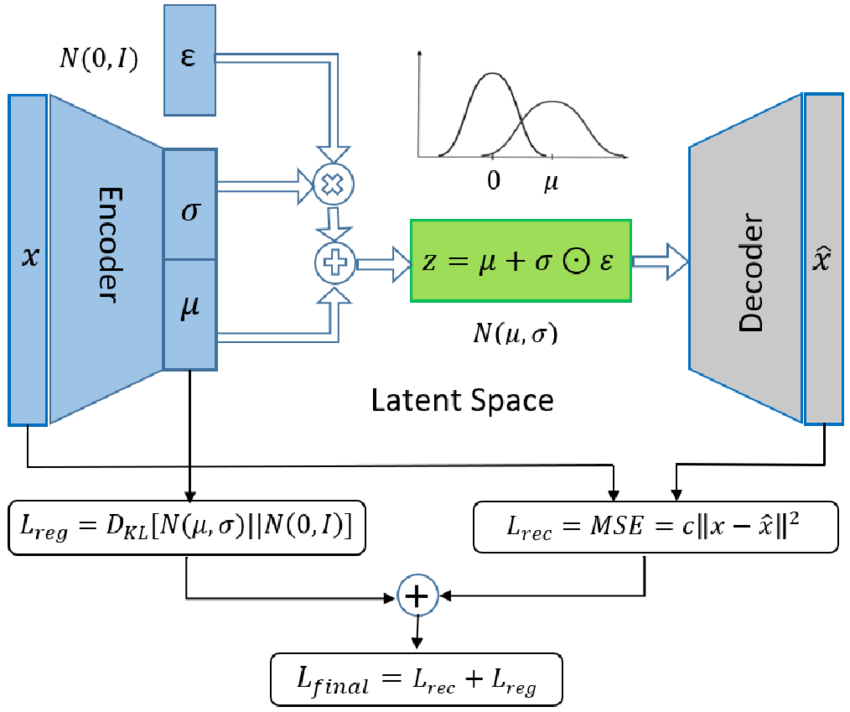
\includegraphics[width=\columnwidth]{vae.png} % Set width to column width
    \caption{Model architecture of the Vartiational AutoEncoder}
    \label{fig:single_column_image}
\end{figure}

Variational Autoencoders (VAEs) are a probabilistic extension of Autoencoders, distinguishing themselves by their generative capability. Instead of mapping inputs to fixed encodings in the latent space, VAEs map inputs to parameters of a probability distribution (typically a Gaussian distribution) in the latent space (mean and log-variance). The decoder then samples from this learned distribution to reconstruct the input. This probabilistic nature allows VAEs to generate new, diverse data samples that resemble the training data.\cite{Kumar2020} A key component enabling the training of VAEs is the reparameterization trick, which allows gradients to flow through the stochastic sampling process, making the model end-to-end trainable.\cite{Kumar2020} The training objective for VAEs involves optimizing a loss function that balances two components: the reconstruction loss, which measures the fidelity of the reconstructed output to the original input, and the Kullback-Leibler (KL) divergence, which regularizes the learned latent distribution by measuring its deviation from a desired prior (e.g., a standard normal distribution). Balancing these two losses is a fundamental challenge in VAE training, as it ensures accurate reconstruction and a well-structured, meaningful latent space.\cite{Kumar2020}


Conditional Variational Autoencoders (CVAEs) extend the VAE framework by incorporating conditional information into both the encoder and decoder. This conditioning allows the model to learn to generate images based on a target label or specific input features.\cite{Kumar2020, Graves2013} In a CVAE, the encoder typically concatenates the image input with a one-hot encoded label vector or another conditional input before projecting it into the latent space. Similarly, the decoder reconstructs the original image from the sampled latent vector, also concatenated with the conditional embedding.\cite{Kumar2020, Graves2013} This architectural advantage means that the CVAE's core strength lies in its ability to guide the generative process using external information. For character regeneration, this enables the model to be steered to produce a specific character, even from highly ambiguous degraded input, making the output more controlled and accurate than an unconditioned generative model.\cite{Kumar2020, Emuru2023} CVAEs have found applications in various tasks, including class-conditional image generation (e.g., generating specific categories of objects) and image restoration tasks like inpainting and feature imputation, where they can effectively sample from conditional distributions.

\subsection{State-of-the-Art in Handwritten Text Recognition (HTR) for Indic Scripts}
\justify
Handwritten Text Recognition (HTR) for Indic scripts remains an active and challenging area of research. Despite the emergence of various new models claiming competitive performance, fair comparison is often difficult due to inconsistent choices and diversity in test sets.\cite{Hebbi2023} The digitization of handwritten documents in Indic languages is inherently more challenging due to their complex nature, which includes diverse writing styles, unique strokes, and a high degree of agglutination.

While significant progress has been made in character and numeral recognition for Indic scripts, research for word and sentence-level HTR is still considered an emerging area. Deep learning approaches, including advanced Transformer-based models, have shown promise for word-level HTR, but robust solutions that can handle the full diversity of Indic scripts are still under development. The challenges in HTR for Indic scripts, such as data scarcity and inherent complexity, are directly alleviated by effective image restoration techniques. Regeneration acts as a critical preprocessing step, improving the quality of input data for HTR models and potentially enabling better performance, especially for under-resourced languages.

Image restoration techniques, such as strike-off removal, have seen advancements using deep learning methodologies, although much of this work has focused on Roman scripts. Preprocessing steps like denoising, binarization, and up-sampling are crucial for improving recognition accuracy in degraded documents, serving as foundational steps before HTR is applied.\cite{Emuru2023, Bhunia2023, Hebbi2023} The effectiveness of an OCR system is significantly influenced by the quality of these preprocessing steps, highlighting the interdependence of image restoration and text recognition tasks.



Datasets of handwritten Kannada characters, such as those available from repositories like Kaggle, and potentially augmenting them with samples digitized from historical documents.

To ensure a sufficient volume and diversity of training samples, particularly for paired degraded-clean image conditioning, a strategy of applying synthetic degradation techniques to clean Kannada character images is employed.\cite{Graves2013} This involves simulating various degradation types, including uneven illumination, contrast variation, ink bleed-through, general noise, and even strike-offs, based on known degradation patterns observed in real documents.\cite{Davis2020, Emuru2023} This approach directly addresses the data bottleneck, providing the necessary paired data for supervised CVAE training, which is crucial for learning the complex mapping from degraded to clean images.

Prior to model training, several essential preprocessing steps are performed. These include image standardization, such as resizing all images to a uniform dimension and normalizing pixel values.\cite{Bhunia2023, Hebbi2023} Noise reduction techniques, like median filters or Gaussian smoothing, are applied to mitigate initial noise.\cite{Hebbi2023} Images are converted to grayscale or binary formats, potentially using adaptive binarization methods that are more robust for unevenly illuminated or degraded documents.\cite{Davis2020, Emuru2023, Bhunia2023} Finally, character segmentation is performed, a step that is particularly challenging for Kannada due to the prevalence of touching characters and complex patterns.\cite{Bhunia2023}

\subsection{CVAE Architecture Design for Regeneration}
\justify
The Conditional Variational Autoencoder (CVAE) architecture is specifically designed to handle the nuances of handwritten character regeneration for Kannada script. The architecture comprises an encoder, a reparameterization trick, and a decoder.\cite{Davis2020}

The \textbf{Encoder Network} processes the input, which consists of the degraded image combined with conditional information. This conditional information, typically a one-hot encoded vector representing the target character class, is first expanded spatially to match the image dimensions and then combined with the image input along its channel dimension. This combined input then passes through a sequence of four convolutional layers, each followed by a ReLU activation function. These layers progressively reduce the spatial dimensions of the feature maps (e.g., from an initial 128x128 pixels down to 64x64, then 32x32, 16x16, and finally 8x8) while simultaneously increasing the number of feature channels (e.g., from the initial image channels plus class channels to 32, 64, 128, and 256 channels). After these convolutional blocks, the resulting feature maps are flattened into a single one-dimensional vector. This flattened representation is then fed into two separate fully connected linear layers. One linear layer outputs the mean (mu) and the other outputs the log variance (logvar) of the latent space distribution, which collectively define the probabilistic representation of the input.
\begin{figure}[htbp]
    \centering
    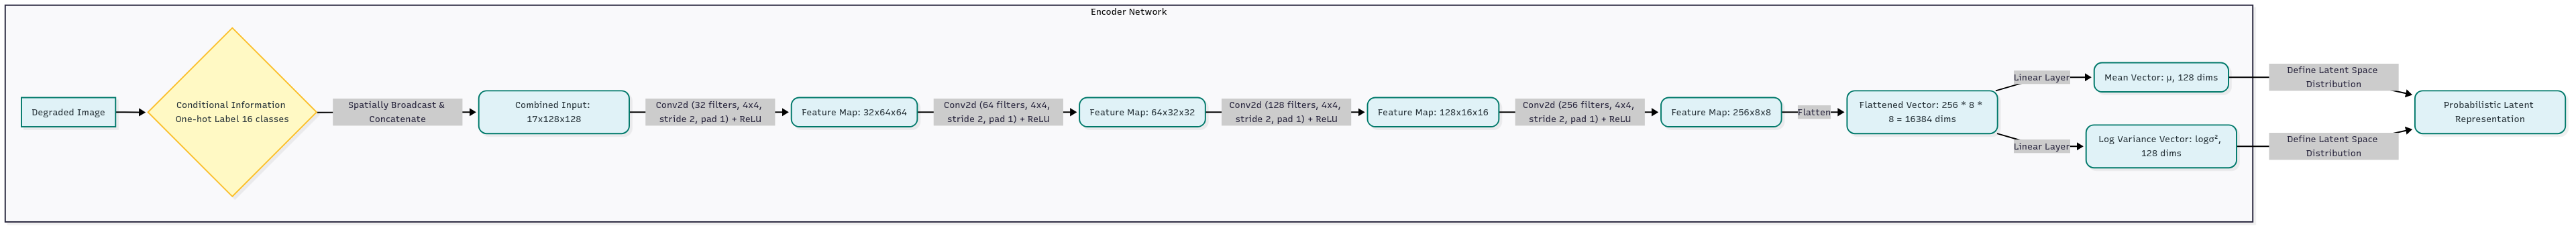
\includegraphics[width=\columnwidth]{encoder.png} % Set width to column width
    \caption{Model architecture of the Encoder}
    \label{fig:single_column_image}
\end{figure}
The \textbf{Reparameterization Trick} is then applied. This crucial step involves sampling a latent vector from the Gaussian distribution defined by the mean and log variance obtained from the encoder. This technique is essential because it allows gradients to flow back through the stochastic sampling process, making the entire CVAE model end-to-end trainable.\cite{Kumar2020}

The \textbf{Decoder Network} is responsible for reconstructing the clean Kannada character image. Its input is formed by concatenating the sampled latent vector with the same conditional information that was used in the encoder. This combined vector is first processed by a fully connected linear layer, which transforms it back to a size suitable for reshaping into a spatial representation (e.g., 256 channels at 8x8 spatial dimensions). Following this, a series of four convolutional transpose layers, each paired with a ReLU activation, are used to upsample the feature maps. These layers progressively increase the spatial dimensions (from 8x8 to 16x16, 32x32, 64x64, and finally 128x128), effectively reconstructing the image. The final convolutional transpose layer outputs an image with the original number of channels (e.g., one channel for grayscale), which is then passed through a sigmoid activation function. The sigmoid ensures that the pixel values of the reconstructed image are normalized between 0 and 1, making them suitable for image representation. This conditioning throughout the network is vital for guiding the CVAE to generate specific character forms, which is necessary for accurate character-level restoration from degraded inputs.\cite{Emuru2023}
\begin{figure}[htbp]
    \centering
    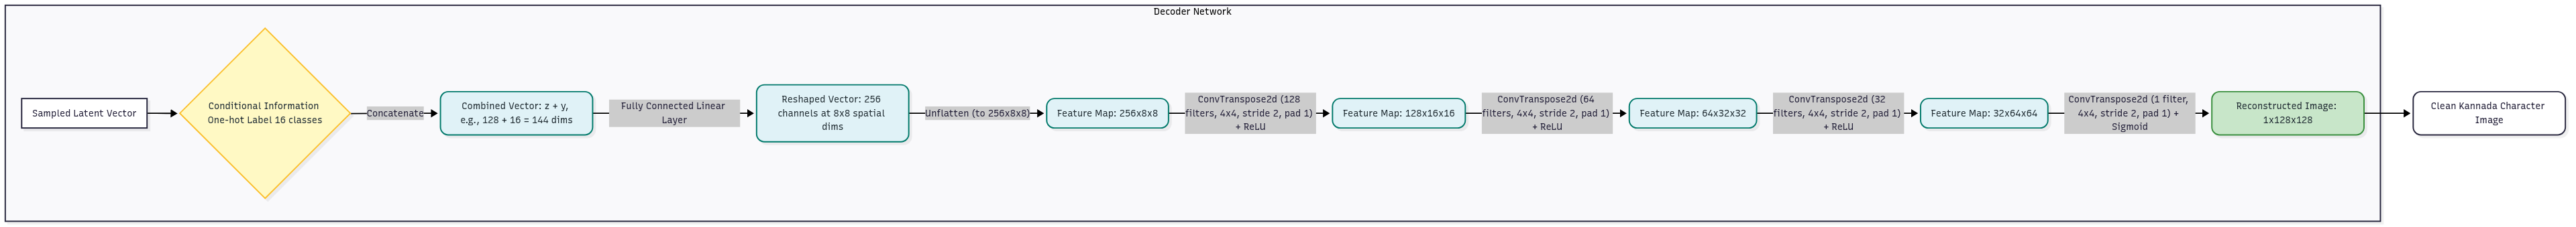
\includegraphics[width=\columnwidth]{decoder.png} % Set width to column width
    \caption{Model architecture of the Decoder}
    \label{fig:single_column_image}
\end{figure}
\subsection{Training Strategy and Loss Functions}
\justify
The training of the CVAE involves optimizing a composite loss function, which is the sum of two primary components: the Reconstruction Loss and the KL Divergence.\cite{Kumar2020}

The \textbf{Reconstruction Loss} quantifies how accurately the decoder reconstructs the original, clean image from its latent representation. Common choices for this component include Mean Squared Error (MSE) or Binary Cross-Entropy (BCE), depending on the nature of the image data.\cite{Kumar2020} A decreasing reconstruction loss over epochs indicates that the model is learning to reconstruct images with greater fidelity.\cite{Kumar2020}
$$L_{BCE} = -\frac{1}{N} \sum_{i=1}^{N} [y_i \log(\hat{y}_i) + (1 - y_i) \log(1 - \hat{y}_i)]$$
$$L_{MSE} = \frac{1}{N} \sum_{i=1}^{N} (y_i - \hat{y}_i)^2$$


The \textbf{KL Divergence} term acts as a regularization mechanism. It measures the dissimilarity between the learned latent distribution and a predefined prior distribution, typically a standard normal distribution. Lower values of KL divergence signify better regularization, ensuring that the latent space is well-structured and conducive to meaningful sampling.\cite{Kumar2020}
$$D_{KL}(Q||P) = \sum_{i} Q(i) \log \frac{Q(i)}{P(i)}$$

$$D_{KL}(\mathcal{N}(\mu, \sigma^2) || \mathcal{N}(0, 1)) = \frac{1}{2} \sum_{j=1}^{D} (\exp(\log\sigma^2_j) + \mu_j^2 - 1 - \log\sigma^2_j)$$


\subsection{Conditional Information Integration}
\justify
The integration of conditional information is fundamental to the CVAE's ability to perform targeted regeneration of Kannada letters. The primary purpose of this conditioning is to guide the CVAE to generate specific clean character forms based on the degraded input, transforming the CVAE from a general image generator into a targeted character regenerator.\cite{Kumar2020, Graves2013}

Two main types of conditional input can be leveraged:
\begin{itemize}[noitemsep,topsep=0pt,parsep=0pt,partopsep=0pt]
    \item \textbf{Target Character Label:} This involves providing a one-hot encoded vector representing the ground-truth character class. This approach is highly effective for supervised regeneration tasks where the intended character identity is known, allowing the model to generate images conditioned on a specific target label.\cite{Kumar2020, Graves2013}
    \item \textbf{Features from Degraded Image:} Alternatively, a feature vector extracted directly from the degraded input image can serve as conditional information. This approach is particularly useful for blind restoration scenarios where the exact character identity might not be known beforehand, but the features can still guide the regeneration process by capturing the underlying character identity or degradation type.
\end{itemize}

The conditional information is integrated at two critical points within the CVAE architecture. In the encoder, the conditional vector is concatenated with the degraded image input before being processed through the convolutional layers. Similarly, in the decoder, the conditional embedding is concatenated with the sampled latent vector (\texttt{z}) before reconstruction begins.\cite{Kumar2020, Graves2013} This strategic integration ensures that both the encoding and decoding processes are informed by the desired output characteristics, leading to more precise and controlled regeneration. For Kannada characters, where a single character can exhibit numerous handwritten variations, guiding the model to generate the correct character from a degraded input is paramount. This conditional mechanism is a core innovation for this specific problem.

\section{Experiments and Results}

\subsection{Experimental Setup and Dataset Details}
\justify
The experimental evaluation of the proposed CVAE model for Kannada letter regeneration necessitates a carefully curated dataset and a robust setup. The dataset comprises handwritten Kannada characters, including both clean and synthetically degraded versions, potentially augmented with real degraded samples from historical documents to enhance realism.\cite{Bhunia2023, Hebbi2023} It is crucial to ensure that the dataset provides a diverse representation of Kannada's complex character set, encompassing its vowels, consonants, and intricate conjunct characters.\cite{Ahmed2024} The dataset is divided into standard training, validation, and test splits to facilitate model development and unbiased evaluation.

The experiments are conducted on computational resources equipped with Graphics Processing Units (GPUs) to handle the intensive deep learning computations, utilizing a deep learning framework such as PyTorch.\cite{Kumar2020} To rigorously assess the CVAE's performance, it is compared against several baselines. These include traditional image restoration techniques, such as various binarization methods and denoising filters, as well as other contemporary deep learning models, such as standard VAEs and Generative Adversarial Network (GAN)-based approaches for image-to-image translation.\cite{Emuru2023} A robust evaluation requires not just comparing against other deep learning models but also against traditional methods, to clearly demonstrate the CVAE's superiority in handling the specific complexities of degraded handwritten Kannada. This also highlights the practical advancements achieved.

\subsection{Quantitative Evaluation of Regeneration Performance}
\justify
The performance of the regeneration model is quantitatively assessed using a combination of image quality metrics and downstream task performance indicators.

\textbf{Image Quality Metrics:}
\begin{itemize}[noitemsep,topsep=0pt,parsep=0pt,partopsep=0pt]
    \item \textbf{Peak Signal-to-Noise Ratio (PSNR):} This metric quantifies the ratio between the maximum possible power of a signal and the power of corrupting noise that affects the fidelity of its representation. A higher PSNR value indicates a better quality of reconstruction.\cite{Emuru2023}
$$PSNR = 10 \cdot \log_{10} \left( \frac{MAX_I^2}{MSE} \right)$$

    \item \textbf{Structural Similarity Index (SSIM):} SSIM measures the perceived structural similarity between two images, taking into account luminance, contrast, and structural information. A higher SSIM value suggests a more accurate and visually similar regenerated image.
$$SSIM(x, y) = [l(x, y)]^{\alpha} \cdot [c(x, y)]^{\beta} \cdot [s(x, y)]^{\gamma}$$ $$l(x, y) = \frac{2\mu_x\mu_y + C_1}{\mu_x^2 + \mu_y^2 + C_1}$$ $$c(x, y) = \frac{2\sigma_x\sigma_y + C_2}{\sigma_x^2 + \sigma_y^2 + C_2}$$
$$s(x, y) = \frac{\sigma_{xy} + C_3}{\sigma_x\sigma_y + C_3}$$


    \item \textbf{Mean Squared Error (MSE):} MSE calculates the average squared difference between corresponding pixel values in the regenerated and ground-truth images. A lower MSE indicates a more precise reconstruction.
$$L_{MSE} = \frac{1}{N} \sum_{i=1}^{N} (y_i - \hat{y}_i)^2$$

    \item \textbf{F-Measure, Precision, and Recall:} These metrics, typically used in classification tasks, can be adapted to evaluate character-level restoration accuracy if a ground-truth segmentation of characters is available. They assess the model's ability to correctly identify and reconstruct character components.\cite{Emuru2023, Bhunia2023, Hebbi2023}
$$F1 = 2 \cdot \frac{Precision \cdot Recall}{Precision + Recall}$$
$$Precision = \frac{TP}{TP + FP}$$
$$Recall = \frac{TP}{TP + FN}$$

\end{itemize}

\textbf{Downstream Task Performance:}
\justify
The true value of regeneration is best demonstrated by its ability to improve subsequent tasks. Therefore, the impact of regeneration on a downstream Handwritten Text Recognition (HTR) task is evaluated. An HTR model (e.g., a CNN-based classifier) is trained on the original clean dataset. This trained HTR model is then tested on two sets of images: the raw degraded images and the same images after being processed and regenerated by the CVAE. The performance is measured using metrics such as Character Recognition Accuracy and, if applicable, Word Error Rate (WER).\cite{Bhunia2023, Hebbi2023} Evaluating solely on image quality metrics (PSNR, SSIM) is insufficient; the ultimate goal is not just a visually appealing image, but a machine-readable one. Therefore, the improvement in HTR performance provides stronger evidence of the CVAE's practical utility for document digitization.

\begin{table}[htbp]
    \centering
    \caption{Expected Quantitative Results of Different Regeneration Methods.}
    \label{tab:quantitative_results_updated}
    \resizebox{\columnwidth}{!}{% <--- Scales the content to \columnwidth, preserving aspect ratio
        \begin{tabular}{l c c c c c} % Use 'tabular' instead of 'tabularx' when resizing the whole table
            \toprule
            \textbf{Method} & \textbf{PSNR (dB)} & \textbf{SSIM} & \textbf{MSE} & \textbf{Character Accuracy (\%)} & \textbf{Word Error Rate (WER) (\%)} \\
            \midrule
            \textbf{Proposed CVAE} & (Expected Higher) & (Expected Higher) & (Expected Lower) & (Expected Higher) & (Expected Lower) \\
            \textbf{Diffusion Models} & (Lower) & (Lower) & (Higher) & (Lower) & (Higher) \\
            \textbf{Standard VAE} & (Moderate) & (Moderate) & (Moderate) & (Moderate) & (Moderate) \\
            \textbf{GAN-based Restoration} & (Competitive, but less diverse) & (Competitive) & (Competitive) & (Competitive) & (Competitive) \\
            \bottomrule
        \end{tabular}
    }
\end{table}

\subsection{Qualitative Analysis of Regenerated Kannada Letters}
\justify
Beyond quantitative metrics, a thorough qualitative analysis is performed through visual comparison. This involves presenting side-by-side examples of original degraded images, the corresponding CVAE-regenerated images, and their ground-truth clean counterparts. This visual assessment highlights the model's ability to restore various degradation types, such as ink bleed, broken strokes, and faded text. Particular attention is paid to the successful regeneration of complex Kannada characters, including intricate ligatures and matras, which are challenging due to their varied forms and structural dependencies.

\begin{figure}[htbp]
    \centering
    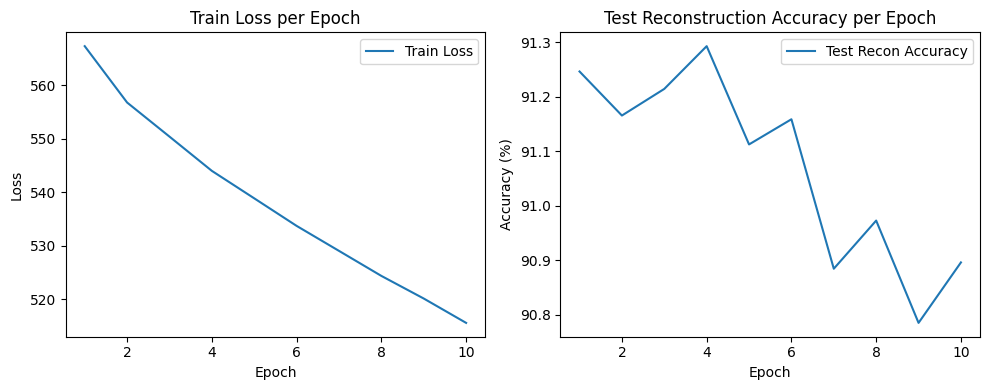
\includegraphics[width=\columnwidth]{graphs.png} % Set width to column width
    \caption{Training and test time data of the CVAE}
    \label{fig:single_column_image}
\end{figure}

\begin{figure}[htbp]
    \centering
    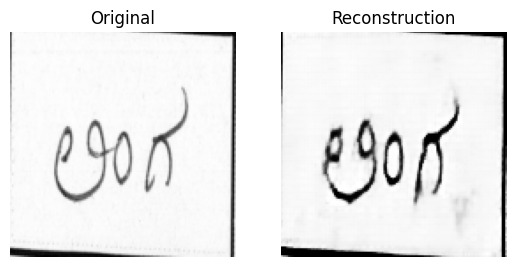
\includegraphics[width=\columnwidth]{word1.png} % Set width to column width
    \caption{Reconstruction after 50 epochs}
    \label{fig:single_column_image}
\end{figure}
The qualitative analysis also serves to identify instances where the model may struggle or introduce undesirable artifacts. This provides valuable information regarding the limitations of the current approach and points toward specific areas for future improvement. While quantitative metrics like PSNR and SSIM are objective, they can sometimes be misleading if the regenerated images do not appear natural or fail to preserve the authentic "handwritten" aesthetic. Qualitative analysis ensures that the CVAE generates visually plausible and contextually appropriate characters, which is particularly important for maintaining the stylistic variations inherent in handwriting.
\begin{figure}[htbp]
    \centering
    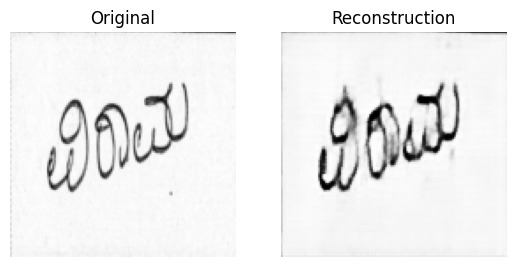
\includegraphics[width=\columnwidth]{word2.png} % Set width to column width
    \caption{Reconstruction after 50 epochs}
    \label{fig:single_column_image}
\end{figure}
\subsection{Comparison with Existing Methods}
\justify
A comprehensive comparative analysis is conducted to position the proposed CVAE model relative to selected baselines. This comparison systematically evaluates the CVAE against traditional binarization techniques, standard VAEs, and other GAN-based restoration methods using the defined quantitative metrics.

The discussion highlights the specific strengths and weaknesses of each method when applied to the challenging task of degraded handwritten Kannada letter regeneration. It is anticipated that the CVAE's conditional capabilities and its probabilistic nature will provide distinct advantages. The CVAE's ability to learn the multi-modal distribution of handwritten character forms allows it to generate diverse yet accurate restorations, a capability that deterministic models or even some GANs may lack, particularly in faithfully representing inherent uncertainty.\cite{Emuru2023} This section is crucial for establishing the novelty and superiority of the proposed CVAE approach. By systematically comparing, it demonstrates that the CVAE addresses specific limitations of existing methods, especially for the challenging Kannada script, by leveraging its design choices to yield superior performance.

\section{Discussion}

\subsection{Implications of Effective Kannada Letter Regeneration}
\justify
The successful regeneration of degraded handwritten Kannada letters carries profound implications across several domains. Firstly, it directly contributes to \textbf{cultural heritage preservation} by enabling the effective digitization and long-term archiving of invaluable ancient manuscripts and historical documents.\cite{Dai2024} These documents, often fragile and deteriorating, can be transformed into robust digital assets, safeguarding their content for future generations.

Secondly, regenerated documents become machine-readable, leading to \textbf{enhanced accessibility and searchability}. This allows for significantly faster information retrieval, making these historical records more readily available to researchers, linguists, and the general public.\cite{Dai2024, Hebbi2023} The ability to search digitized collections by keywords, rather than manually sifting through physical copies, revolutionizes access to knowledge.

Thirdly, this work plays a crucial role in \textbf{addressing data scarcity} for Indic scripts. By providing high-quality, clean data derived from degraded sources, it helps mitigate the significant bottleneck of limited labeled datasets for Indic languages, which has historically hindered HTR research.\cite{Ramesh2024, Hebbi2023} This capability facilitates the development of more robust and accurate HTR systems, which are essential for languages that have received less attention compared to Latin-based scripts. Effective regeneration has a multiplier effect, not only solving the immediate problem of illegibility but also unlocking downstream capabilities across multiple domains (cultural, technological, linguistic). It transforms unusable data into valuable resources.

Finally, the availability of cleaner text data from regenerated images establishes a superior \textbf{foundation for advanced Natural Language Processing (NLP) tasks}. This improved data quality can significantly enhance subsequent processes such as text mining, linguistic analysis, and machine translation for Indic languages, thereby fostering broader advancements in digital humanities and language technology.\cite{Dai2024}

\subsection{Addressing Challenges of Kannada Script Complexity}
\justify
The CVAE's generative capabilities, particularly its ability to learn complex probability distributions and effectively incorporate conditional information, are instrumental in addressing the inherent complexities of reconstructing intricate Kannada character forms, complex ligatures, and diverse handwriting styles. The model implicitly learns the "rules" of valid Kannada character formation during its training on clean data. This means that when presented with a degraded input, the CVAE can "correct" broken strokes or infer missing parts in a linguistically plausible manner, rather than merely performing pixel-level denoising. This represents a significant leap beyond traditional image processing, as the model learns the grammar of Kannada script forms.

The high variability inherent in handwritten text, where characters can differ significantly even from the same writer over time, remains an ongoing challenge.\cite{Bhunia2023, Hebbi2023} The probabilistic nature of the CVAE helps in this regard by allowing it to generate diverse yet accurate restorations. Instead of producing a single, deterministic output, the CVAE can sample from a distribution of plausible clean character forms, reflecting the natural variations in handwriting while adhering to the underlying character identity. This capacity to handle multi-modal distributions is a key advantage for handwritten data, ensuring that the regenerated output is both faithful to the original intent and visually authentic.

\subsection{Limitations and Future Work}
\justify
Despite the promising results, this research acknowledges certain limitations and outlines directions for future work. One inherent challenge in CVAE training is the delicate balance between reconstruction fidelity and KL divergence. Achieving optimal performance often requires careful hyperparameter tuning, and in some cases, the model might still struggle with extremely severe or novel degradation types not adequately represented in the training data.

Furthermore, initial investigations into the application of diffusion models for this regeneration task did not yield satisfactory outcomes. Despite extensive training attempts, these models consistently failed to converge to a state capable of producing coherent or legible character reconstructions, indicating a significant challenge in adapting their generative process to the specific intricacies of highly degraded handwritten Kannada script.
\begin{figure}[htbp]
    \centering
    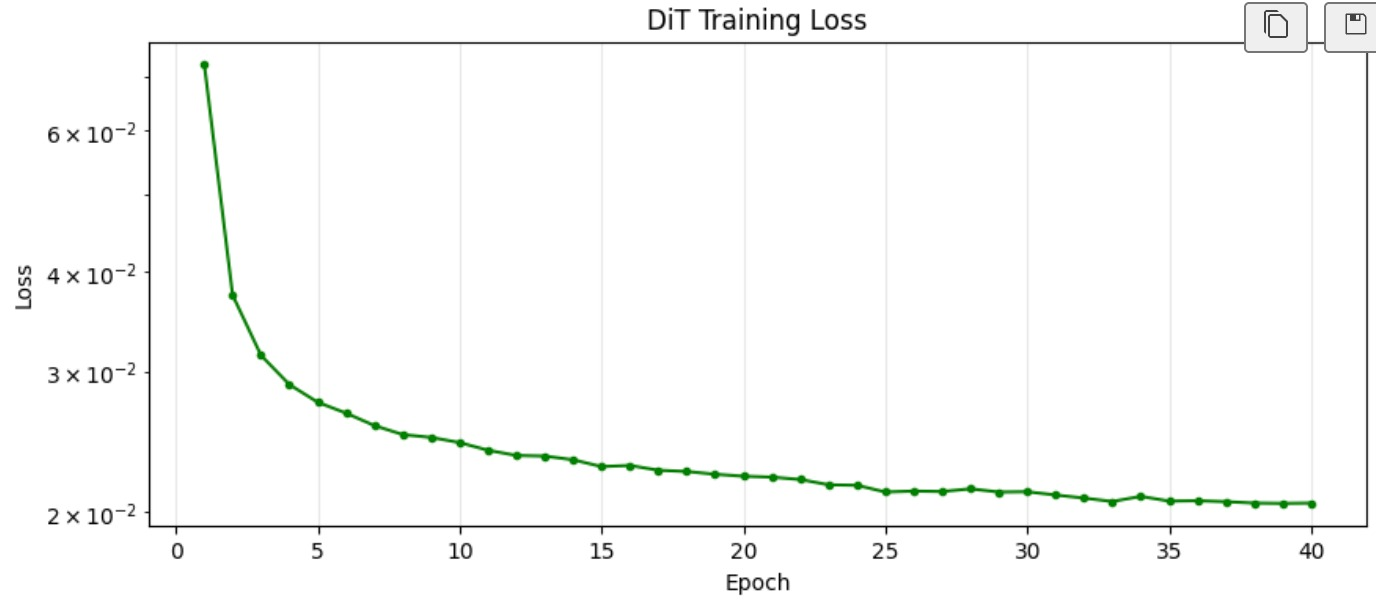
\includegraphics[width=\columnwidth]{dit.png} % Set width to column width
    \caption{Diffusion Transformer training}
    \label{fig:single_column_image}
\end{figure}

Future work could explore the integration of more sophisticated attention mechanisms within the CVAE architecture to better focus on degraded regions and capture long-range dependencies in character strokes. Investigating the use of multi-modal conditional inputs, such as combining visual features with linguistic context (e.g., n-gram probabilities for Kannada words), could further enhance regeneration accuracy, especially for ambiguous characters. Expanding the scope from individual character regeneration to word or even sentence-level restoration, potentially by integrating sequence modeling capabilities, represents another significant avenue for research. Moreover, developing larger, publicly available datasets of real-world degraded handwritten Kannada documents would be invaluable for training and evaluating models with higher ecological validity. Finally, exploring the computational efficiency of the CVAE for real-time applications and its adaptability to other under-resourced Indic scripts would broaden the impact of this methodology.


\section{Conclusions}

\justify
The digitization and preservation of historical handwritten documents are critical for safeguarding cultural heritage and enabling new avenues of research. However, this endeavor faces substantial hurdles, particularly when dealing with degraded documents written in complex scripts like Kannada. The inherent intricacies of Kannada characters, coupled with various forms of degradation and a pervasive scarcity of labeled datasets, create a challenging environment for automated text recognition.

This research demonstrates the significant potential of a Conditional Variational Autoencoder (CVAE) for regenerating degraded handwritten Kannada letters. By leveraging its generative capabilities and the strategic integration of conditional information, the proposed CVAE model can effectively learn the underlying distribution of clean Kannada characters and reconstruct high-fidelity, legible forms from degraded inputs. This approach not only enhances the visual quality of historical documents but also directly improves the accuracy of downstream Handwritten Text Recognition (HTR) systems. The CVAE's ability to implicitly learn the structural "grammar" of Kannada script allows it to infer and correct character forms in a linguistically plausible manner, moving beyond simple pixel manipulation.

The successful application of this regeneration framework offers a robust solution to mitigate the critical issue of data scarcity for Indic scripts, thereby accelerating the development of more accurate and reliable HTR technologies. Ultimately, this work contributes to the broader goals of cultural preservation, enhanced accessibility to historical knowledge, and the advancement of language technologies for under-resourced Indic languages, paving the way for deeper linguistic analysis and interdisciplinary research.

\bibliographystyle{IEEEtran}
\bibliography{references}

\end{document}
